\chapter{TINJAUAN PUSTAKA}
\label{bab:tinjauan-pustaka}

Bab ini membahas landasan teori yang mendukung pemilihan data, arsitektur, dan cara evaluasi. Pembahasan mencakup kategori kerusakan jalan, keluarga YOLO, modifikasi arsitektur dan pembobotan kelas, serta generalisasi lintas domain. Penelitian terkait digunakan untuk menjelaskan posisi evaluasi komparatif yang dilakukan.

\section{Kerusakan Permukaan Jalan dan Dataset}
\subsection{Kategori kerusakan dan objek permukaan jalan}
Dalam deteksi berbasis citra, objek direpresentasikan melalui kategori dan kotak pembatas. RDD2022 menggunakan empat kelas kerusakan, yaitu retak memanjang (D00), retak melintang (D10), retak buaya (D20), dan lubang jalan (D40)~\cite{Arya2024846}. Retak memanjang dan melintang dibedakan menurut arah pola retaknya. Retak buaya membentuk pola retak saling terhubung, sedangkan lubang menunjukkan bagian permukaan yang mengalami kehilangan material.

Penutup saluran dan tambalan juga dapat muncul pada citra jalan. Kedua objek tersebut memiliki karakteristik visual yang perlu dibedakan dari lubang. Matouq dkk. menempatkan lubang, penutup saluran, dan tambalan sebagai kategori yang perlu dipertimbangkan bersama~\cite{matouq2024ai}. Pada penelitian ini, istilah kelas pengecoh menyatakan peran D70 dan D80 dalam pengujian kebingungan visual. Istilah tersebut tidak menyatakan bahwa setiap tambalan berada dalam kondisi baik atau tidak memerlukan pemeriksaan.

Hubungan kategori dengan perannya dalam penelitian ditunjukkan pada Tabel~\ref{tab:kategori}.
\begin{table}[H]
\centering
\caption{Kategori sumber yang digunakan dalam penelitian.}
\label{tab:kategori}
\begingroup\fontsize{10}{13}\selectfont
\begin{tabularx}{\linewidth}{|l|X|X|}\hline
\rowcolor{black}\HeaderTabel{Kode}&\HeaderTabel{Kategori}&\HeaderTabel{Peran dalam evaluasi}\\\hline
D00 & Retak memanjang & Kerusakan inti\\\hline
D10 & Retak melintang & Kerusakan inti\\\hline
D20 & Retak buaya & Kerusakan inti\\\hline
D40 & Lubang jalan & Kerusakan inti\\\hline
D70 & Penutup saluran (\textit{manhole}) & Kelas pengecoh\\\hline
D80 & Jalan bertambal (\textit{patchy road}) & Kelas pengecoh\\\hline
\end{tabularx}\endgroup
\end{table}
Tabel~\ref{tab:kategori} memisahkan empat kelas kerusakan dari dua kelas tambahan. Pemisahan ini menjadi dasar perbandingan pelatihan empat dan enam kelas, serta penyamaan kategori pada evaluasi lintas domain.

\subsection{RDD2022 dan N-RDD2024}
RDD2022 merupakan dataset lintas negara yang mencakup Jepang, India, Tiongkok, Ceko, Norwegia, dan Amerika Serikat~\cite{Arya2024846}. Keragaman sumber memungkinkan pengujian pada citra dengan kondisi berbeda. Namun, komposisi negara dan kategori pada dataset tetap membatasi cakupan bukti yang dihasilkan. Kinerja agregat tidak otomatis menggambarkan kemampuan detektor di seluruh wilayah.

N-RDD2024 memperluas anotasi menjadi sepuluh kategori~\cite{kaya2024nrdd2024}. Selain empat kategori kerusakan utama, terdapat retak diperbaiki, pejalan kaki, marka, penutup saluran, jalan bertambal, dan alur roda. Penelitian ini mengambil enam kategori sebagaimana Tabel~\ref{tab:kategori} dari subset Asia. Pembatasan tersebut menyediakan data untuk membandingkan detektor pada kerusakan inti sekaligus objek yang berpotensi menyerupai lubang.

Jumlah anotasi antarkelas dapat berbeda. Dalam deteksi objek, banyaknya citra dan banyaknya objek merupakan dua ukuran yang berbeda karena satu citra dapat memiliki beberapa anotasi. Analisis distribusi karena itu perlu menghitung objek per kelas, bukan hanya citra. Distribusi data latih digunakan untuk pembobotan kelas, sedangkan data validasi dan uji dipertahankan untuk fungsi evaluasinya.

\section{Deteksi Objek dengan Keluarga YOLO}
\subsection{Prinsip deteksi satu tahap}
YOLO merumuskan deteksi objek melalui jaringan yang memprediksi lokasi dan kategori objek dalam satu proses komputasi maju~\cite{redmon2016you}. Pendekatan satu tahap menghindari kebutuhan proposal wilayah terpisah pada alur prediksi. Keluaran detektor mencakup kotak pembatas, kelas, dan nilai kepercayaan. Nilai kepercayaan digunakan dalam penyaringan prediksi, tetapi tidak boleh langsung dimaknai sebagai kepastian bahwa objek benar-benar ada.

Pada detektor modern, rincian representasi kotak dan cara pemilihan prediksi dapat berbeda. Oleh karena itu, mekanisme kisi pada YOLO awal tidak digunakan sebagai penjelasan identik untuk semua varian. Dalam penelitian ini, keluarga YOLO dipilih sebagai dasar perbandingan karena tersedia model bawaan serta modifikasi untuk citra jalan~\cite{Li2024,Zeng2024,Wang2025}.

\subsection{Komponen utama YOLOv8}
YOLOv8 dapat dijelaskan melalui tiga komponen, yaitu \textit{backbone}, \textit{neck}, dan \textit{head}~\cite{Li2024,Zeng2024}. \textit{Backbone} mengekstraksi fitur dari citra. \textit{Neck} memadukan fitur pada beberapa resolusi agar informasi spasial dan semantik dapat digunakan bersama. \textit{Head} menghasilkan prediksi lokasi dan kelas berdasarkan fitur tersebut.

Pada YOLOv8, struktur ekstraksi fitur mencakup konvolusi, blok C2f, dan SPPF. Penggabungan fitur menggunakan operasi perubahan resolusi dan konkatenasi. Kepala deteksi memisahkan pengolahan klasifikasi dan regresi lokasi~\cite{Li2024,Zeng2024}. Arsitektur dasar tersebut ditunjukkan pada Gambar~\ref{fig:yolo-konseptual}.
\begin{figure}[H]
\centering
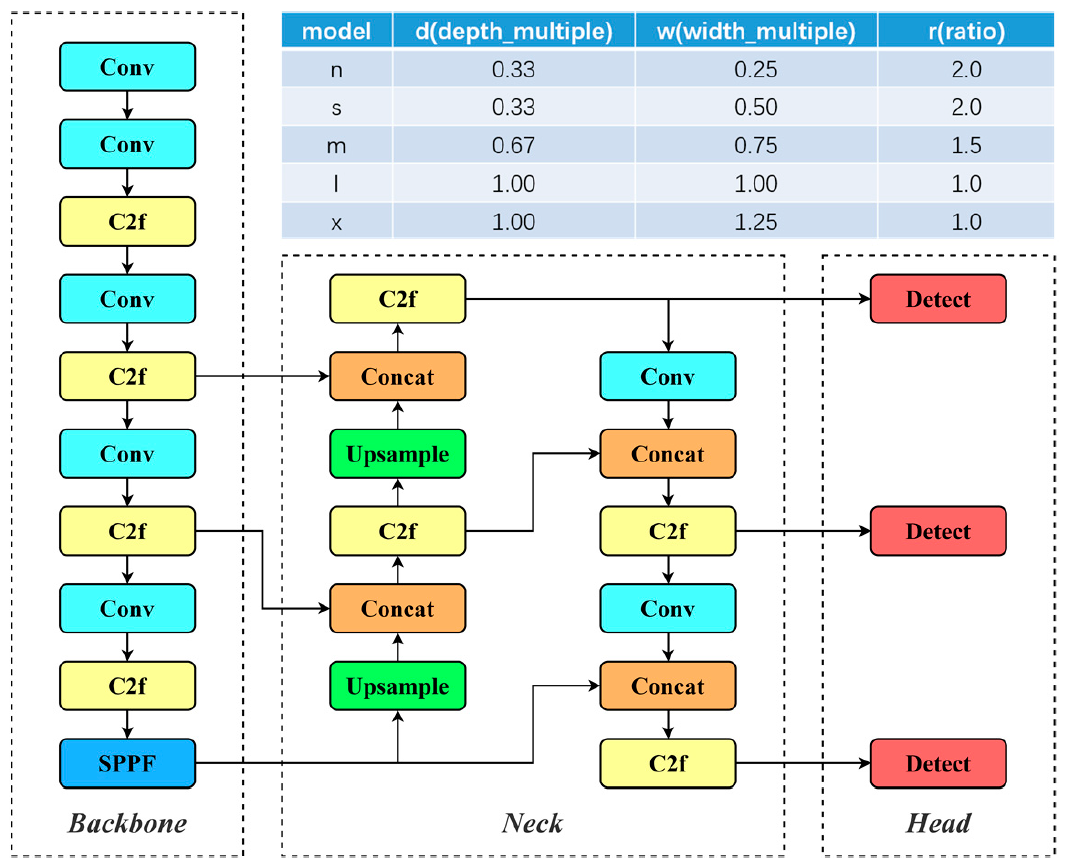
\includegraphics[width=.95\linewidth]{arsitektur_yolov8_standar.png}
\caption[Arsitektur dasar YOLOv8.]{Arsitektur dasar YOLOv8, digunakan kembali dari proposal; sumber Li dkk.~\cite{Li2024}.}
\label{fig:yolo-konseptual}
\end{figure}
Gambar~\ref{fig:yolo-konseptual} menunjukkan hubungan komponen YOLOv8 dan pilihan penskalaan jaringannya. Gambar ini digunakan untuk membedakan lokasi perubahan arsitektur pada ekstraksi fitur, penggabungan fitur, dan kepala deteksi.

\textit{Non-maximum suppression} (NMS) digunakan pada detektor yang memerlukan penyaringan kotak bertumpang tindih. Proses ini mempertimbangkan nilai kepercayaan dan tumpang tindih spasial. Ambang NMS memiliki fungsi berbeda dari ambang pencocokan prediksi dengan anotasi pada evaluasi. Perbedaan ini perlu dijaga agar aturan pascapemrosesan tidak tertukar dengan definisi keberhasilan deteksi.

\subsection{Varian pembanding}
YOLOv8n digunakan sebagai model dasar. YOLOv12n mewakili rancangan berbasis atensi yang dibahas oleh Tian dkk.~\cite{tian2025yolov12_primary}. YOLO26n menjadi pembanding lain dengan jalur deteksi \textit{end-to-end} yang berbeda~\cite{sapkota2025yolo26_primary}. Perbedaan tersebut berarti seluruh model tidak harus menggunakan langkah pascapemrosesan yang sama.

YOLOv8-PD dan YOLO-RD mewakili modifikasi yang dikembangkan untuk deteksi kerusakan jalan~\cite{Zeng2024,Wang2025}. Kedua model diterapkan melalui rekonstruksi lokal. Dengan demikian, pembanding penelitian adalah implementasi yang digunakan, bukan hasil reproduksi identik perangkat lunak penulis asli. Penskalaan nano pada model-model tersebut juga tidak menjamin kesamaan kapasitas jaringan.

\section{Modifikasi Arsitektur dan Pembobotan Kelas}
\subsection{Konvolusi ringan dan mekanisme atensi}
Konvolusi ringan bertujuan mengurangi kebutuhan operasi atau parameter pada pembentukan fitur. GhostNet memanfaatkan sejumlah fitur dasar dan transformasi yang lebih murah untuk menghasilkan fitur tambahan~\cite{han2020ghostnet}. Gagasan tersebut menjadi salah satu dasar penggunaan blok berbasis Ghost dalam model ringan. Efisiensi aktualnya tetap bergantung pada susunan jaringan dan perangkat eksekusi.

Mekanisme atensi mengatur kontribusi fitur secara adaptif. Dalam penelitian kerusakan jalan, atensi digunakan untuk membantu pengolahan informasi objek di antara tekstur latar yang kompleks~\cite{Li2024,Zeng2024}. Penerapan modul atensi tidak selalu mengurangi kebutuhan komputasi. Manfaat yang dilaporkan pada suatu penelitian juga tidak dapat langsung dipindahkan ke dataset atau implementasi lain.

YOLOv8-PD menggabungkan komponen berbasis Ghost, pengolahan atensi, dan kepala deteksi dengan berbagi konvolusi~\cite{Zeng2024}. YOLO-RD menggunakan modul operasi bintang, penyempurnaan atensi, dan pengolahan berbasis wavelet~\cite{Wang2025}. Komponen ini menjadi dasar rekonstruksi dalam penelitian. Penjelasan perbedaan rekonstruksi dan konfigurasi aktual ditempatkan pada Bab~\ref{bab:perancangan-sistem}.

\subsection{Ketimpangan kelas dan jumlah efektif sampel}
Ketimpangan kelas terjadi ketika frekuensi kategori pada data pelatihan tidak seimbang. Pembobotan kelas merupakan salah satu pendekatan untuk mengubah kontribusi kategori terhadap fungsi kerugian. Cui dkk. merumuskan jumlah efektif sampel berdasarkan gagasan bahwa tambahan informasi tidak selalu bertambah secara linear terhadap jumlah sampel~\cite{cui2019class}.

Jumlah efektif kelas $c$ dituliskan pada Persamaan~\eqref{eq:effective-number}.
\begin{equation}
E_c=\frac{1-\beta^{n_c}}{1-\beta}.
\label{eq:effective-number}
\end{equation}
Pada Persamaan~\eqref{eq:effective-number}, $n_c$ menyatakan jumlah sampel kelas $c$ dan $\beta$ berada pada rentang $0\leq\beta<1$. Penelitian ini mengoperasionalkan $n_c$ sebagai jumlah anotasi objek pada data latih. Kebalikan $E_c$ menjadi dasar bobot kelas. Normalisasi yang diterapkan dalam implementasi dirumuskan pada Persamaan~\eqref{eq:class-weight}.
\begin{equation}
a_c=\frac{1-\beta}{1-\beta^{n_c}},\qquad
w_c=\frac{K a_c}{\sum_{j=1}^{K}a_j}.
\label{eq:class-weight}
\end{equation}
Persamaan~\eqref{eq:class-weight} menghasilkan bobot $w_c$ dengan rata-rata satu untuk $K$ kelas pelatihan. Bobot dihitung hanya dari data latih. Pemisahan ini mencegah penggunaan frekuensi target untuk menentukan kontribusi kelas selama pelatihan sumber.

\subsection{Penerapan pada komponen klasifikasi}
Pembobotan tersebut diterapkan pada komponen \textit{binary cross-entropy} (BCE) untuk klasifikasi. Secara konseptual, bentuk berbobotnya dinyatakan pada Persamaan~\eqref{eq:weighted-bce}.
\begin{equation}
\ell_{ic}=-w_c\left[y_{ic}\log p_{ic}+(1-y_{ic})\log(1-p_{ic})\right].
\label{eq:weighted-bce}
\end{equation}
Pada Persamaan~\eqref{eq:weighted-bce}, $p_{ic}$ adalah probabilitas prediksi kelas $c$ pada posisi prediksi $i$. Simbol $y_{ic}$ menyatakan target klasifikasi, yang dapat berupa skor hasil penugasan target detektor. Persamaan ini menjelaskan kontribusi bobot pada klasifikasi; agregasi, normalisasi, dan komponen regresi mengikuti implementasi detektor.

Intervensi pada penelitian ini menggunakan $\beta=0{,}999$. Pembobotan berbasis frekuensi tersebut berbeda dari penambahan faktor modulasi berdasarkan kesulitan prediksi pada \textit{Focal Loss}. Karena eksperimen utama memakai pembobotan yang sama, hasilnya tidak digunakan untuk mengklaim keunggulan pembobotan atas fungsi kerugian lain. Klaim demikian memerlukan perbandingan khusus yang mengisolasi perubahan fungsi kerugian.

\section{Generalisasi dan Evaluasi Deteksi}
\subsection{Domain sumber, target, dan pengujian zero-shot}
Domain sumber adalah distribusi data yang digunakan untuk melatih model, sedangkan domain target merupakan lingkungan evaluasi yang berbeda. Penelitian deteksi kerusakan lintas negara menunjukkan bahwa kinerja perlu diperiksa pada kondisi di luar data sumber~\cite{arya2021deep,Arya2024846}. Perbedaan distribusi dapat melibatkan tampilan citra maupun komposisi objek.

Dalam penelitian ini, \textit{zero-shot} berarti penerapan model terlatih pada domain target tanpa \textit{fine-tuning}. Istilah ini merujuk pada perpindahan domain untuk kategori yang telah dikenal selama pelatihan. Pengujian tersebut bukan deteksi kategori baru yang sama sekali tidak tersedia pada data sumber.

Perbandingan lintas domain harus menggunakan himpunan kelas yang sama. Jika sumber dirata-ratakan atas enam kelas dan target atas lima kelas, selisih metrik turut dipengaruhi oleh perbedaan kategori. Penelitian ini karena itu memisahkan hasil enam kelas sumber dari perbandingan empat kelas kerusakan yang tersedia pada kedua domain. Selisih kinerja menjadi ukuran deskriptif pada dua himpunan data, tanpa mengidentifikasi penyebabnya secara kausal.

\subsection{Pencocokan kotak dan metrik deteksi}
\textit{Intersection over union} (IoU) mengukur tumpang tindih antara kotak prediksi $B_p$ dan kotak anotasi $B_g$~\cite{Li2024,Zeng2024}. Rumusnya ditunjukkan pada Persamaan~\eqref{eq:iou}.
\begin{equation}
\operatorname{IoU}(B_p,B_g)=\frac{|B_p\cap B_g|}{|B_p\cup B_g|}.
\label{eq:iou}
\end{equation}
Persamaan~\eqref{eq:iou} membandingkan luas irisan dengan luas gabungan kedua kotak. Nilainya digunakan untuk menentukan kecocokan spasial pada ambang tertentu. Untuk evaluasi per kelas, prediksi juga harus sesuai dengan kategori anotasi.

Prediksi yang cocok secara kelas dan lokasi disebut \textit{true positive} (TP). Prediksi yang tidak memperoleh pasangan valid dihitung sebagai \textit{false positive} (FP), sedangkan anotasi yang tidak terdeteksi menjadi \textit{false negative} (FN). Pencocokan membatasi penggunaan pasangan sehingga beberapa prediksi pada objek yang sama tidak semuanya dihitung benar. Berdasarkan hitungan tersebut, presisi dan \textit{recall} dirumuskan pada Persamaan~\eqref{eq:pr}.
\begin{equation}
P=\frac{TP}{TP+FP},\qquad R=\frac{TP}{TP+FN}.
\label{eq:pr}
\end{equation}
Persamaan~\eqref{eq:pr} membedakan ketepatan prediksi positif ($P$) dari kemampuan menemukan objek beranotasi ($R$). Keduanya berubah mengikuti ambang kepercayaan yang digunakan. F1 menyatukan kedua ukuran melalui rata-rata harmonis, seperti pada Persamaan~\eqref{eq:f1}.
\begin{equation}
F1_c=\frac{2P_cR_c}{P_c+R_c},\qquad
F1_{\mathrm{macro}}=\frac{1}{K}\sum_{c=1}^{K}F1_c.
\label{eq:f1}
\end{equation}
Pada Persamaan~\eqref{eq:f1}, $K$ adalah jumlah kelas yang dievaluasi. F1 bernilai nol ketika jumlah presisi dan \textit{recall} nol. Rata-rata makro memberikan kontribusi yang sama kepada setiap kelas, sehingga tidak didominasi langsung oleh kelas dengan anotasi terbanyak.

\textit{Average precision} (AP) merangkum kurva presisi--\textit{recall} ketika ambang kepercayaan berubah. Rata-rata AP antarkelas menghasilkan mAP~\cite{Li2024,Wu2023}, sebagaimana Persamaan~\eqref{eq:map}.
\begin{equation}
\operatorname{mAP}_{K}=\frac{1}{K}\sum_{c=1}^{K}AP_c.
\label{eq:map}
\end{equation}
Persamaan~\eqref{eq:map} digunakan dengan himpunan kelas yang dinyatakan secara eksplisit. mAP@0,5 menggunakan ambang IoU 0,5. mAP@0,5:0,95 merata-ratakan AP pada sepuluh ambang IoU dari 0,5 sampai 0,95 dengan langkah 0,05. Metrik kedua mempertimbangkan tuntutan ketepatan lokasi yang lebih beragam.

\subsection{Ukuran efisiensi komputasi}
Jumlah parameter menggambarkan banyaknya parameter dalam representasi model yang dihitung. GFLOPs menyatakan perkiraan miliaran operasi titik mengambang untuk satu komputasi maju pada ukuran masukan tertentu. GFLOPs bukan jumlah operasi per detik. Ukuran ini perlu dibedakan dari kecepatan aktual karena jenis operasi dan implementasi perangkat lunak turut berpengaruh~\cite{Wu2023}.

FPS menyatakan banyaknya citra yang dapat diproses per detik menurut prosedur pengukuran. Dalam penelitian ini, FPS diestimasi dari jumlah rerata waktu prapemrosesan, inferensi, dan pascapemrosesan per citra. Metrik tersebut tidak mencakup seluruh alur aplikasi, seperti akuisisi video dan penyajian antarmuka. Karena itu, FPS digunakan sebagai pembanding pada lingkungan uji yang tercatat.

\section{Penelitian Terkait dan Posisi Penelitian}
Penelitian terdahulu menyediakan dasar pemilihan model serta pertanyaan evaluasi. RDD-YOLO membahas pengembangan YOLOv8 dengan SimAM dan GhostConv~\cite{Li2024}. YOLOv8-PD menekankan rancangan ringan berbasis YOLOv8n~\cite{Zeng2024}, sedangkan YOLO-RD mengembangkan pemrosesan fitur untuk deteksi kerusakan~\cite{Wang2025}. Ketiganya menjadi rujukan untuk menilai ketepatan dan kebutuhan komputasi secara bersama.

Kajian Matouq dkk. memberi dasar untuk memperhatikan kategori penutup saluran dan tambalan dalam deteksi lubang~\cite{matouq2024ai}. Sementara itu, penelitian Hugo dkk. menggunakan citra jalan Indonesia untuk mengevaluasi EfficientDet~\cite{hugo2025efficientdet}. Penelitian tersebut mendukung kebutuhan evaluasi lokal, tetapi protokolnya berbeda dari transfer tanpa pelatihan ulang yang digunakan di sini. Ringkasan keterkaitannya disajikan pada Tabel~\ref{tab:penelitian-terkait}.

\begin{table}[H]
\centering
\caption{Penelitian terkait dan keterkaitannya dengan penelitian ini.}
\label{tab:penelitian-terkait}
\begingroup\fontsize{10}{13}\selectfont
\begin{tabularx}{\linewidth}{|p{2.5cm}|X|X|}\hline
\rowcolor{black}\HeaderTabel{Penelitian}&\HeaderTabel{Fokus}&\HeaderTabel{Keterkaitan}\\\hline
Li dkk.~\cite{Li2024} & RDD-YOLO pada RDD2022; atensi dan konvolusi ringan & Dasar pembahasan modifikasi YOLO untuk citra jalan\\\hline
Zeng dan Zhong~\cite{Zeng2024} & YOLOv8-PD untuk deteksi kerusakan jalan & Dasar rekonstruksi model berorientasi efisiensi\\\hline
Wang dkk.~\cite{Wang2025} & YOLO-RD dengan pengembangan ekstraksi fitur & Dasar rekonstruksi model pembanding\\\hline
Matouq dkk.~\cite{matouq2024ai} & Deteksi lubang beserta objek permukaan terkait & Motivasi pengujian label pengecoh\\\hline
Hugo dkk.~\cite{hugo2025efficientdet} & EfficientDet pada citra jalan Indonesia & Konteks evaluasi pada data lokal\\\hline
Arya dkk.~\cite{arya2021deep,Arya2024846} & Dataset dan evaluasi lintas negara & Dasar pengujian generalisasi antardomain\\\hline
\end{tabularx}\endgroup
\end{table}
Tabel~\ref{tab:penelitian-terkait} menghubungkan literatur dengan keputusan penelitian, tanpa menjadikan skor dari dataset berbeda sebagai peringkat langsung. Perbandingan dalam TA ini menggunakan data sumber yang sama, implementasi yang terdokumentasi, dan evaluasi target tanpa penyesuaian bobot.

Posisi penelitian adalah evaluasi bersama terhadap model dasar, model berbasis pengembangan arsitektur, dan rekonstruksi model khusus kerusakan jalan. Pengujian label pengecoh melengkapi perbandingan tersebut. Kontribusinya terletak pada karakterisasi kinerja implementasi dan generalisasi pada target lokal, bukan pada klaim penemuan arsitektur baru atau keunggulan universal suatu model.
